\swjtuChapter{系统测试报告}

% 去掉章节前缀，使用 1 / 1.1 / 1.1.1 的编号体系
\setcounter{section}{0}
\renewcommand{\thesection}{\arabic{section}}
\renewcommand{\thesubsection}{\thesection.\arabic{subsection}}
\renewcommand{\thesubsubsection}{\thesubsection.\arabic{subsubsection}}

\section{项目简介}

\subsection{项目业务功能介绍}
系统业务覆盖“顾客购前导购、购中结算、购后库存联动”全链路，核心流程如下：
\begin{enumerate}[leftmargin=2em]
  \item 顾客通过小程序进行文本检索或图片识别，定位目标商品。
  \item 顾客将商品加入购物车并发起结算。
  \item 后端校验库存并生成订单，写入库存日志与告警信息。
  \item 管理员在管理端维护商品与摄像头，并通过巡检调度监控货架状态。
\end{enumerate}

\begin{center}
  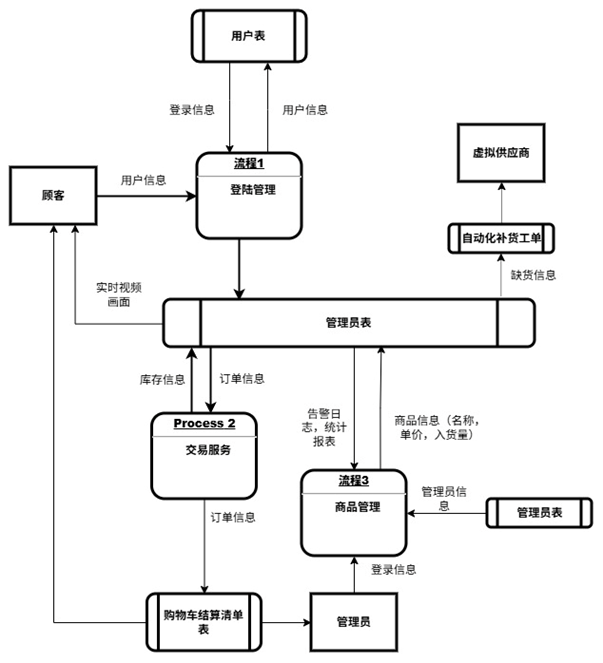
\includegraphics[width=0.9\textwidth]{images/图3-8.png}\\[0.3em]
  {\zihao{-5}图4-1\quad 系统顶层数据流（测试对象边界）}
\end{center}

\subsection{术语及主要名称介绍}
\begin{itemize}[leftmargin=2em]
  \item \textbf{白盒测试}：基于代码逻辑路径的测试方法，关注语句、条件、路径覆盖。
  \item \textbf{黑盒测试}：基于需求输入输出的测试方法，关注功能行为与边界。
  \item \textbf{冒烟测试}：以最小用例集合快速验证核心流程可用性。
  \item \textbf{基线路径}：选取系统中最关键、最高频的业务路径进行持续回归。
\end{itemize}

\subsection{参考文献}
\begin{enumerate}[leftmargin=2em]
  \item 《软件测试的艺术》
  \item ISTQB 基础级测试标准
  \item Postman 官方文档
  \item JMeter 官方文档
\end{enumerate}

\section{测试需求说明}

\subsection{编写目的}
本文档用于明确测试范围、测试策略、测试环境与验收标准，确保系统交付前在功能正确性、稳定性与可维护性方面满足课程项目要求。

\subsection{系统功能需求}
本轮测试覆盖以下功能域：
\begin{itemize}[leftmargin=2em]
  \item 登录鉴权（管理端与小程序）。
  \item 商品管理（分页、增删改、图片上传）。
  \item 购物车与订单结算（加购、结算、订单查询、支付）。
  \item 库存告警（生成、分页查询、处理）。
  \item 摄像头与巡检调度（绑定、预览、手动触发、参数更新）。
  \item AI 接口联动（文本检索、中心识别、批量识别）。
\end{itemize}

\subsection{非功能性需求指标}
\begin{center}
  \renewcommand{\arraystretch}{1.35}
  \zihao{5}
  \begin{tabular}{|>{\centering\arraybackslash}m{2.8cm}|>{\centering\arraybackslash}m{4.0cm}|>{\centering\arraybackslash}m{5.4cm}|}
    \hline
    \textbf{指标类别} & \textbf{目标值} & \textbf{说明} \\ \hline
    接口响应 & 常规接口 P95 \textless= 200ms & 在本地联调网络下，剔除图片上传与视频流场景 \\ \hline
    识别能力 & 单帧推理时延可控、结果稳定返回 & 重点验证接口可用性与字段完整性 \\ \hline
    一致性 & 订单与库存同事务提交 & 失败时必须回滚，避免脏数据 \\ \hline
    可恢复性 & 异常时返回统一错误结构 & 全局异常处理器输出 \texttt{code/message/data} \\ \hline
  \end{tabular}
  \\[0.3em]
  {\zihao{-5}表4-1\quad 非功能性测试指标}
\end{center}

\subsection{环境需求}
\begin{itemize}[leftmargin=2em]
  \item 操作系统：Windows 10/11。
  \item JDK：21。
  \item Maven：3.9+。
  \item Python：3.10+，依赖 \texttt{fastapi/uvicorn/opencv-python/numpy/pydantic}。
  \item Node.js：18+（项目当前环境为 Node.js 24）。
  \item 数据库与缓存：MySQL 8.x、Redis 8.x。
  \item 客户端工具：Postman、微信开发者工具。
\end{itemize}

\subsection{测试人员要求}
\begin{enumerate}[leftmargin=2em]
  \item 熟悉 RESTful 接口测试、HTTP 状态码与 JSON 结构校验。
  \item 能阅读 Java/Python 关键业务代码，完成白盒路径分析。
  \item 能使用 Postman/JMeter 执行功能与性能测试。
\end{enumerate}

\subsection{测试标准}
\begin{itemize}[leftmargin=2em]
  \item 关键业务链路（登录、加购、结算、告警）必须通过。
  \item 高风险缺陷（导致数据错误或流程中断）必须关闭。
  \item 非阻断类问题可带条件上线，但需有规避方案与修复计划。
\end{itemize}

\section{测试计划}

本次测试采用“先冒烟后回归”的策略：
\begin{enumerate}[leftmargin=2em]
  \item \textbf{阶段一：接口冒烟测试}，验证主流程可跑通。
  \item \textbf{阶段二：白盒路径覆盖}，针对结算、鉴权、巡检等核心代码进行路径分析和用例补齐。
  \item \textbf{阶段三：黑盒方法测试}，按等价类、边界值、判定表、场景法执行回归。
  \item \textbf{阶段四：性能与异常测试}，验证可用性与容错性。
\end{enumerate}

入口条件：后端、AI、数据库、缓存服务已启动；初始化数据已导入。  
退出条件：主流程缺陷清零，回归用例通过率满足验收要求。

\section{测试过程及用例}

\subsection{白盒测试用例}
白盒测试聚焦 \texttt{OrderServiceImpl.checkout}、\texttt{JwtAuthInterceptor.preHandle}、\texttt{CameraScanScheduler.executeScanBatchTask} 三条关键链路。

\subsubsection{语句覆盖}
\begin{center}
  \renewcommand{\arraystretch}{1.35}
  \zihao{5}
  \begin{tabular}{|>{\centering\arraybackslash}m{1.8cm}|>{\centering\arraybackslash}m{4.0cm}|>{\centering\arraybackslash}m{5.8cm}|}
    \hline
    \textbf{用例ID} & \textbf{测试目标} & \textbf{预期结果} \\ \hline
    WB-S-01 & 用户未登录直接结算 & 返回 401，流程中止 \\ \hline
    WB-S-02 & 购物车为空结算 & 返回 400，提示购物车为空 \\ \hline
    WB-S-03 & 库存充足正常结算 & 生成订单、写入明细、库存扣减成功 \\ \hline
    WB-S-04 & AI 批量识别调用异常 & 返回 502，调度任务记录错误日志 \\ \hline
  \end{tabular}
  \\[0.3em]
  {\zihao{-5}表4-2\quad 白盒语句覆盖用例}
\end{center}

\subsubsection{条件覆盖}
\begin{itemize}[leftmargin=2em]
  \item 条件 C1：\texttt{userId == null || userId < 1}
  \item 条件 C2：\texttt{goods.stock < quantity}
  \item 条件 C3：\texttt{remainStock < 10}
\end{itemize}

对应条件覆盖用例如下：
\begin{center}
  \renewcommand{\arraystretch}{1.35}
  \zihao{5}
  \begin{tabular}{|>{\centering\arraybackslash}m{1.8cm}|>{\centering\arraybackslash}m{3.3cm}|>{\centering\arraybackslash}m{3.0cm}|>{\centering\arraybackslash}m{3.5cm}|}
    \hline
    \textbf{用例ID} & \textbf{输入场景} & \textbf{覆盖条件} & \textbf{预期结果} \\ \hline
    WB-C-01 & 无 Token 请求 & C1=True & 返回 401 \\ \hline
    WB-C-02 & 库存不足下单 & C2=True & 事务回滚，返回库存不足 \\ \hline
    WB-C-03 & 库存临界值下单 & C3=True & 订单成功且生成告警 \\ \hline
    WB-C-04 & 库存充足下单 & C1/C2/C3=False & 订单成功，无告警 \\ \hline
  \end{tabular}
  \\[0.3em]
  {\zihao{-5}表4-3\quad 白盒条件覆盖用例}
\end{center}

\subsubsection{基本路径覆盖}
以结算模块构建控制流图后选取 4 条基本路径：
\begin{enumerate}[leftmargin=2em]
  \item P1：未登录路径（入口即失败）。
  \item P2：购物车为空路径（参数通过但业务拦截）。
  \item P3：库存不足路径（中途失败并回滚）。
  \item P4：成功路径（订单与库存均提交，异步清空购物车）。
\end{enumerate}

\subsection{黑盒测试用例}

\subsubsection{等价类划分}
\begin{center}
  \renewcommand{\arraystretch}{1.35}
  \zihao{5}
  \begin{tabular}{|>{\centering\arraybackslash}m{2.2cm}|>{\centering\arraybackslash}m{3.2cm}|>{\centering\arraybackslash}m{4.6cm}|>{\centering\arraybackslash}m{3.2cm}|}
    \hline
    \textbf{功能} & \textbf{有效等价类} & \textbf{无效等价类} & \textbf{判定} \\ \hline
    登录 & username/password 非空且匹配 & 用户名空、密码空、账号不存在、密码错误 & 返回 200/401/400 \\ \hline
    文本检索 & keyword 非空，k\textgreater=1 & keyword 为空，k\textless1 & 返回商品列表或 400 \\ \hline
    商品新增 & name/price/stock/shelfId 合法 & 关键字段缺失或类型非法 & 返回 200 或 400 \\ \hline
  \end{tabular}
  \\[0.3em]
  {\zihao{-5}表4-4\quad 黑盒等价类设计}
\end{center}

\subsubsection{边界值测试}
边界值选取：\texttt{page=1}、\texttt{size=1}、\texttt{k=1}、\texttt{k=100}、\texttt{stock=0}。  
预期：边界内可处理，越界返回参数错误或空结果。

\subsubsection{判定表法}
以“是否允许结算”为例构建判定表：
\begin{itemize}[leftmargin=2em]
  \item 条件：已登录 / 购物车非空 / 库存充足。
  \item 动作：允许结算并生成订单 / 拒绝并给出原因。
\end{itemize}

规则结论：仅当三个条件同时满足时执行结算；任一条件不满足均返回失败。

\subsubsection{因果图法}
因：低库存触发阈值（库存 \textless 安全库存）  
果：生成告警记录，并在管理端待处理列表可见。  
验证点：告警类型、消息文本、状态字段是否正确。

\subsubsection{场景法}
端到端场景 S1：
\begin{enumerate}[leftmargin=2em]
  \item 小程序登录。
  \item 文本检索商品并加入购物车。
  \item 发起结算并支付。
  \item 管理端查看订单与告警变化。
\end{enumerate}

S1 预期：订单生成成功；库存扣减；低库存商品触发告警。

\subsubsection{正交实验法}
针对“搜索体验”选取三因素进行组合：
\begin{itemize}[leftmargin=2em]
  \item 因素 A：搜索方式（文本/图片）。
  \item 因素 B：返回数量 k（3/10/20）。
  \item 因素 C：网络状态（正常/弱网）。
\end{itemize}

通过正交组合验证搜索稳定性与可用性，减少全排列测试成本。

\subsection{性能测试}

本轮性能测试采用“轻量压测 + 接口基准”方式：
\begin{itemize}[leftmargin=2em]
  \item 工具：Postman Runner（基准）、JMeter（并发脚本）。
  \item 对象：\texttt{/api/goods/page}、\texttt{/api/order/checkout}、\texttt{/api/applet/search/text}。
  \item 指标：平均响应时间、P95、错误率。
\end{itemize}

阶段性结论：当前版本已完成单用户和小并发基准验证，系统无阻断性错误；大并发压测建议在独立性能环境继续执行。

\subsection{其他测试}
\begin{itemize}[leftmargin=2em]
  \item \textbf{异常测试}：非法 JSON、错误 Content-Type、未授权 Token。
  \item \textbf{兼容性测试}：管理端 Chrome 浏览器、小程序开发者工具。
  \item \textbf{恢复测试}：AI 服务不可用、Redis 不可用时的降级与报错行为。
  \item \textbf{安全测试}：鉴权拦截、越权访问、敏感错误信息屏蔽。
\end{itemize}

\section{测试报告及分析}

\subsection{测试报告}
基于本阶段用例执行与联调记录，可得结论：
\begin{enumerate}[leftmargin=2em]
  \item 核心业务链路（登录、检索、加购、结算、告警）可闭环运行。
  \item 后端统一异常处理机制有效，错误返回结构一致。
  \item 事务型结算逻辑能够在库存不足场景下回滚，避免数据不一致。
\end{enumerate}

\subsection{缺陷报告}
\begin{center}
  \renewcommand{\arraystretch}{1.35}
  \zihao{5}
  \begin{tabular}{|>{\centering\arraybackslash}m{1.6cm}|>{\centering\arraybackslash}m{4.8cm}|>{\centering\arraybackslash}m{2.5cm}|>{\centering\arraybackslash}m{3.0cm}|}
    \hline
    \textbf{编号} & \textbf{缺陷描述} & \textbf{严重级别} & \textbf{状态} \\ \hline
    BUG-01 & 管理中心点识别返回结果未去重，同一商品被 YOLO 多次检测后在前端重复展示，导致加减购操作出现数量不一致 & 高 & 已修复 \\ \hline
    BUG-02 & AI 识别接口在并发或模型冷启动时偶发超时（原读取超时仅 10 秒），表现为"识别失败请重试" & 高 & 已修复 \\ \hline
    BUG-03 & 小程序查询页增减购操作无法将物品数量减至 0，且每次加入购物车需二次确认后才生效 & 中 & 已修复 \\ \hline
    BUG-04 & 登录页"我们的服务"区域 car 与 search 图标引用路径后缀为 .jpg，而实际文件为 .png，导致图标无法加载显示 & 低 & 已修复 \\ \hline
    BUG-05 & 小程序登录演示环境固定 \texttt{test\_code}，未接入真实 \texttt{code2Session} & 中 & 已知限制 \\ \hline
    BUG-06 & 管理员密码采用 BCrypt 加密存储，历史明文密码已通过自动迁移机制升级 & 低 & 已修复 \\ \hline
  \end{tabular}
  \\[0.3em]
  {\zihao{-5}表4-5\quad 主要缺陷汇总}
\end{center}

\subsection{分析总结}
\begin{itemize}[leftmargin=2em]
  \item 系统在课程项目目标范围内具备可交付性，功能链路完整。已修复的 4 项缺陷覆盖了识别去重、AI 服务容错、前端交互体验和资源加载四个维度。
  \item 当前主要风险集中于"生产级安全与工程化能力"（如微信真实登录对接），不影响课程演示，但需在后续版本中处理。
  \item 识别链路已实现 Python 侧与 Java 侧双端去重 + 前后端双重试机制，可靠性显著提升。
  \item 下一阶段建议补齐自动化测试（JUnit + 前端 E2E）与专项性能压测报告，提升回归效率与可信度。
\end{itemize}
